%%%%%%%%%%%%%%%%%%%%%%%%%%%%%%%%%%%%%%%%%%%%%%%%%%%%%%%%%%%%%
% Programmer : Joseph Vitale
% Date : 02/15/21
% Assessment : CDR Puzzle Me Chess
%%%%%%%%%%%%%%%%%%%%%%%%%%%%%%%%%%%%%%%%%%%%%%%%%%%%%%%%%%%%%

\documentclass[11pt]{article}

%%%%%%%%%%%%%%%%%%%%%%%%%%%%%%%%%%%%%%%%%%%%%%%%%%%%%%%%%%%%%
% Change "article" to "report" to get rid of page number on title page
% Most of these packages that you are calling will be installed by MiKTeX the first time you use it
% After that, they should work fine on your jump drive or laptop
%%%%%%%%%%%%%%%%%%%%%%%%%%%%%%%%%%%%%%%%%%%%%%%%%%%%%%%%%%%%%

\usepackage{amsmath,amsfonts,amsthm,amssymb}
\usepackage{setspace}
\usepackage{Tabbing}
\usepackage{fancyhdr}
\usepackage{lastpage}
\usepackage{extramarks}
\usepackage{chngpage}
\usepackage{soul,color}
\usepackage{graphicx,float,wrapfig}
\usepackage{graphicx}
\usepackage{xcolor}
\usepackage{listings}
\lstset { %
    language=C++,
    backgroundcolor=\color{black!5}, % set backgroundcolor
    basicstyle=\footnotesize,% basic font setting
    }
\graphicspath{ {images/} }

%%%%%%%%%%%%%%%%%%%%%%%%%%%%%%%%%%%%%%%%%%%%%%%%%%%%%%%%%%%%%
% In case you need to adjust margins:
\topmargin=-0.45in      %
\evensidemargin=0in     %
\oddsidemargin=0in      %
\textwidth=6.5in        %
\textheight=9.0in       %
\headsep=0.25in         %
%
%%%%%%%%%%%%%%%%%%%%%%%%%%%%%%%%%%%%%%%%%%%%%%%%%%%%%%%%%%%%%
%%%%%%%%%%%%%%%%%%%%%%%%%%%%%%%%%%%%%%%%%%%%%%%%%%%%%%%%%%%%%
% Homework Specific Information (THIS IS WHERE YOU MAKE YOUR TITLE CHANGES)
%
% You only need to change the homework number and the Date
%
% You should make sure your correct name is on this as well.
%
\newcommand{\hmwkTitle}{Puzzle Me Chess}
\newcommand{\hmwkDueDate}{February\ 22,\ 2021}
\newcommand{\hmwkClass}{Critical Design Review}
\newcommand{\hmwkClassInstructor}{EN.525.743.8VL.SP21}
\newcommand{\hmwkAuthorName}{Mr. Joseph Vitale}

%
%
%
%%%%%%%%%%%%%%%%%%%%%%%%%%%%%%%%%%%%%%%%%%%%%%%%%%%%%%%%%%%%%
%%%%%%%%%%%%%%%%%%%%%%%%%%%%%%%%%%%%%%%%%%%%%%%%%%%%%%%%%%%%%
% Set up for the header and footer here
% This stuff should not change much for you, but you may play around with it safely.
% Notice that the "\lhead" is for the left header and "\chead" is for the center header, etc.

\pagestyle{fancy}                                                      
\lhead{\hmwkAuthorName}                                                 
\chead{\hmwkClass\ (\hmwkClassInstructor )}  
\rhead{\firstxmark}                                                     
\lfoot{\lastxmark}                                                      
\cfoot{}                                                                
\rfoot{Page\ \thepage\ of\ \pageref{LastPage}}                          
\renewcommand\headrulewidth{0.4pt}                                      
\renewcommand\footrulewidth{0.4pt}   
                                   

%%%%%%%%%%%%%%%%%%%%%%%%%%%%%%%%%%%%%%%%%%%%%%%%%%%%%%%%%%%%%
% Tools to mark the numbering of problems. They don't need to be modified by you.
% All the text below is pretty important for the formatting, but you don't need to change it.
%
\newcommand{\enterProblemHeader}[1]{\nobreak\extramarks{#1}{#1 continued on next page\ldots}\nobreak%
                                    \nobreak\extramarks{#1 (continued)}{#1 continued on next page\ldots}\nobreak}%
\newcommand{\exitProblemHeader}[1]{\nobreak\extramarks{#1 (continued)}{#1 continued on next page\ldots}\nobreak%
                                   \nobreak\extramarks{#1}{}\nobreak}%

\newlength{\labelLength}
\newcommand{\labelAnswer}[2]
  {\settowidth{\labelLength}{#1}%
   \addtolength{\labelLength}{0.25in}%
   \changetext{}{-\labelLength}{}{}{}%
   \noindent\fbox{\begin{minipage}[c]{\columnwidth}#2\setlength{\parindent}{10mm}\end{minipage}}%
   \marginpar{\fbox{#1}}%

   % You can leave this alone too
   \changetext{}{+\labelLength}{}{}{}}%

% Nothing to change here
\setcounter{secnumdepth}{0}
\newcommand{\homeworkProblemName}{}%
\newcounter{homeworkProblemCounter}%
\newenvironment{homeworkProblem}[1][Problem \arabic{homeworkProblemCounter}]%
  {\stepcounter{homeworkProblemCounter}%
   \renewcommand{\homeworkProblemName}{#1}%
   \section{\homeworkProblemName}%
   \enterProblemHeader{\homeworkProblemName}}%
  {\exitProblemHeader{\homeworkProblemName}}%

\newcommand{\problemAnswer}[1]
  {\noindent\fbox{\begin{minipage}[c]{\columnwidth}#1\setlength{\parindent}{10mm}\end{minipage}}}%

\newcommand{\problemLAnswer}[1]
  {\labelAnswer{\homeworkProblemName}{#1}}

\newcommand{\homeworkSectionName}{}%
\newlength{\homeworkSectionLabelLength}{}%
\newenvironment{homeworkSection}[1]%
  {% The author put this space here to make sure it is not connected to the above.
   % Otherwise the changetext can do funny things to the other margin

   \renewcommand{\homeworkSectionName}{#1}%
   \settowidth{\homeworkSectionLabelLength}{\homeworkSectionName}%
   \addtolength{\homeworkSectionLabelLength}{0.25in}%
   \changetext{}{-\homeworkSectionLabelLength}{}{}{}%
   \subsection{\homeworkSectionName}%
   \enterProblemHeader{\homeworkProblemName\ [\homeworkSectionName]}}%
  {\enterProblemHeader{\homeworkProblemName}%

   % The author put the blank space above in order to make sure this margin
   % change doesn't happen too soon (otherwise \sectionAnswer's can
   % get ugly about their \marginpar placement.
   \changetext{}{+\homeworkSectionLabelLength}{}{}{}}%

\newcommand{\sectionAnswer}[1]
  {% The author put this space here to make sure we're disconnected from the previous
   % passage

   \noindent\fbox{\begin{minipage}[c]{\columnwidth}#1\setlength{\parindent}{10mm}\end{minipage}}%
   \enterProblemHeader{\homeworkProblemName}\exitProblemHeader{\homeworkProblemName}%
   \marginpar{\fbox{\homeworkSectionName}}%

   % The author put the blank space above in order to make sure this
   % \marginpar gets correctly placed.
   }%
%
% All the text above is pretty important for the formatting, but you don't need to change it.
%
%%%%%%%%%%%%%%%%%%%%%%%%%%%%%%%%%%%%%%%%%%%%%%%%%%%%%%%%%%%%%


%%%%%%%%%%%%%%%%%%%%%%%%%%%%%%%%%%%%%%%%%%%%%%%%%%%%%%%%%%%%%
%    Formatting the title. This part of the document is where the title page is set up.
%    We are almost to the beginning of the homework!
%
\title{\vspace{2in}\textmd{\textbf{\hmwkClass:\ \hmwkTitle}}\\\normalsize\vspace{0.1in}\small{\hmwkDueDate}\\\vspace{0.1in}\large{\textit{\hmwkClassInstructor\ }}\vspace{3in}}
\date{}
\author{\textbf{\hmwkAuthorName}}

%
%
%
%%%%%%%%%%%%%%%%%%%%%%%%%%%%%%%%%%%%%%%%%%%%%%%%%%%%%%%%%%%%%
%%%%%%%%%%%%%%%%%%%%%%%%%%%%%%%%%%%%%%%%%%%%%%%%%%%%%%%%%%%%%
%%%%%%%%%%%%%%%%%%%%%%%%%%%%%%%%%%%%%%%%%%%%%%%%%%%%%%%%%%%%%
%  This is the BEGINNING of the DOCUMENT
%
%
\begin{document}

\maketitle % Actually calling the typesetter to include the title that you formatted above
\newpage
% Comment out the \tableofcontents and \newpage lines to get remove the Contents page
% Uncomment the \setcounter line as well if you do NOT want subsections
%       listed in Contents
%\setcounter{tocdepth}{1}

\tableofcontents % 
%\newpage % The \\ command tells LaTeX to start a new line. 

% When problems are long, it may be desirable to put a \newpage or a
% \clearpage before each homeworkProblem environment

\clearpage 
% The \clearpage command ends the current page and causes all figures 
% and tables that have so far appeared in the input to be printed.
%%%%%%%%%%%%%%%%%%%%%%%%%%%%%%%%%%%%%%%%%%%%%%%%%%%%%%%%%%%%%%%%%%%%%%%%%%%%%%%%%%%%%%%%%%%%%%%%%%%%%%%%%%%%%%%%%%
\section{Project description}
In chess there are many different ways to play the game. After each player moves three times there are 121 million different moves that can end the game. Many people need to practice chess in order to get better and there are many ways to do this. You can play over the internet and play computer which range from (400 - 3200) EIO or you can play puzzle's in chess. Puzzle's in chess allow you to study the board in a given state and make the next several moves. This project is dedicated to solving puzzles in the physical world. 
\\

\noindent The physical chess puzzle allows the user to practice looking at a physical board to solve each puzzle. This project is titled "Puzzle me Chess`` and it will be equipped to have 3 different puzzle's. The chess board will allow the user to place each piece in the right location that is displayed on the OLED screen. After each piece is on the board the chess puzzle will then display to the user which color he/she will play. After the user makes his first move the board will check to see if the move was correct. If not the user will be asked to reset the piece and try again until puzzle is complete. 

\subsection{Capabilities}
Capabilites for the Puzzle me Chess project range from Indicators, User Direction, SD card capability, and Location Detection. See below for more details. More detailed explanation can be found in table \ref{tab:capability}.

\begin{table}
\begin{center}
    \begin{tabular}{| l | l |}
    \hline
    Capability  & Description below\\ \hline
    Indicator &  LED light indicator to show user hint/show answer feature \\ \hline
    User Direction & OLED to describe to the user where to put pieces \\ \hline 
    SD Card & Read .csv standardized format to quickly import puzzles \\ \hline
    User Direction & User input switch to show user answer, indicated by LEDs \\ \hline
    User Direction & User input Button to show user a hint \\ \hline
    Location Detection & Check board spots are correct for puzzle that was selected \\ \hline
    \end{tabular}
    \caption{Shows the Capability's for Puzzle me Chess}
	\label{tab:capability}
\end{center}
\end{table}

\subsection{Assumptions}
Table \ref{tab:Assumptions} shows the assumptions that are being made for this project. The assume were made to reduce overall cost of the project and difficulty to lower risk. 

\begin{table}
\begin{center}
    \begin{tabular}{| l | l |}
    \hline
    Assumptions & Description below\\ \hline
    User Implication  & User puts right pieces on each spot \\ \hline
    Physical &  Chess Board will be lit evenly with light  \\ \hline
    Text File & Each file added to the SDcard will be in a standardized format \\ \hline     
    \end{tabular}
    \caption{Shows the Assumptions that were made for Puzzle me Chess}
	\label{tab:Assumptions}
\end{center}
\end{table}

 
\subsection{Limitations}
Limitations for the Puzzle me Chess project range from Location Detection, Auto Movement, Puzzle Selection, Physical and Physical parts. See table \ref{tab:limitations} for more details.

\begin{table}
\begin{center}
    \begin{tabular}{| l | l |}
    \hline
    Limitations  & Description below\\ \hline
    Location Detection & Not knowing which piece is on the spot \\ \hline
    Auto Movement & Not being able to move the piece on correct spot \\ \hline 
    Puzzle Selection & Not having 3+ different puzzles to choose from  \\ \hline
    Physical & Not being able to light each square along the perimeter  \\ \hline
    Physical Parts & Not having multiple colors to indicate wrong or right answer \\ \hline
    Physical & Needing light to illuminate  the chess board \\ \hline
    \end{tabular}
    \caption{Shows the Limitation's for Puzzle me Chess}
	\label{tab:limitations}
\end{center}
\end{table}

\section{Functional description}
The Puzzle me Chess project will feature a microcontroller, one 21x21 wooden chess board, 8 Multiplexers, 1 switch, 1 Potentiometer, 1 button, and A Display. Figure \ref{fig:Circuit} shows  the current circuit layout as of 02/16/2021, this circuit doesn't show the chess board. Explanation of the System Block Diagram to follow.

\begin{figure}
  \includegraphics[width=\linewidth]{./Pics/Circuit_as_of_2162020.jpg}
  \caption{Circuit layout as of 02/16/2021}
  \label{fig:Circuit}
\end{figure}

\subsection{System Block Diagram}
Figure \ref{fig:SBD1} shows the sudo hand drawn block diagram. The project consist of One Microcontroller which will feature the teensy 3.6, 8 Multiplexer's from Texas Instruments part \# CD4051BE, 1 basic breadboard switch, 1 breadboard Potentiometer, 1 basic breadbaord button, LED's, Photoresister's, 1 Chess Board and one Display. 
\\


\noindent The Chess board will have 1 LED and 1 photoresister per block. The LED will be drilled and placed on the top left side of each block and will be used to show the user where to place each piece. The photoresister will be drilled in the middle of each block and will be used as a voltage drop to tell if there is a piece there or not. See section multiplexer circuit diagram for the circuit layout. 

\begin{figure}
  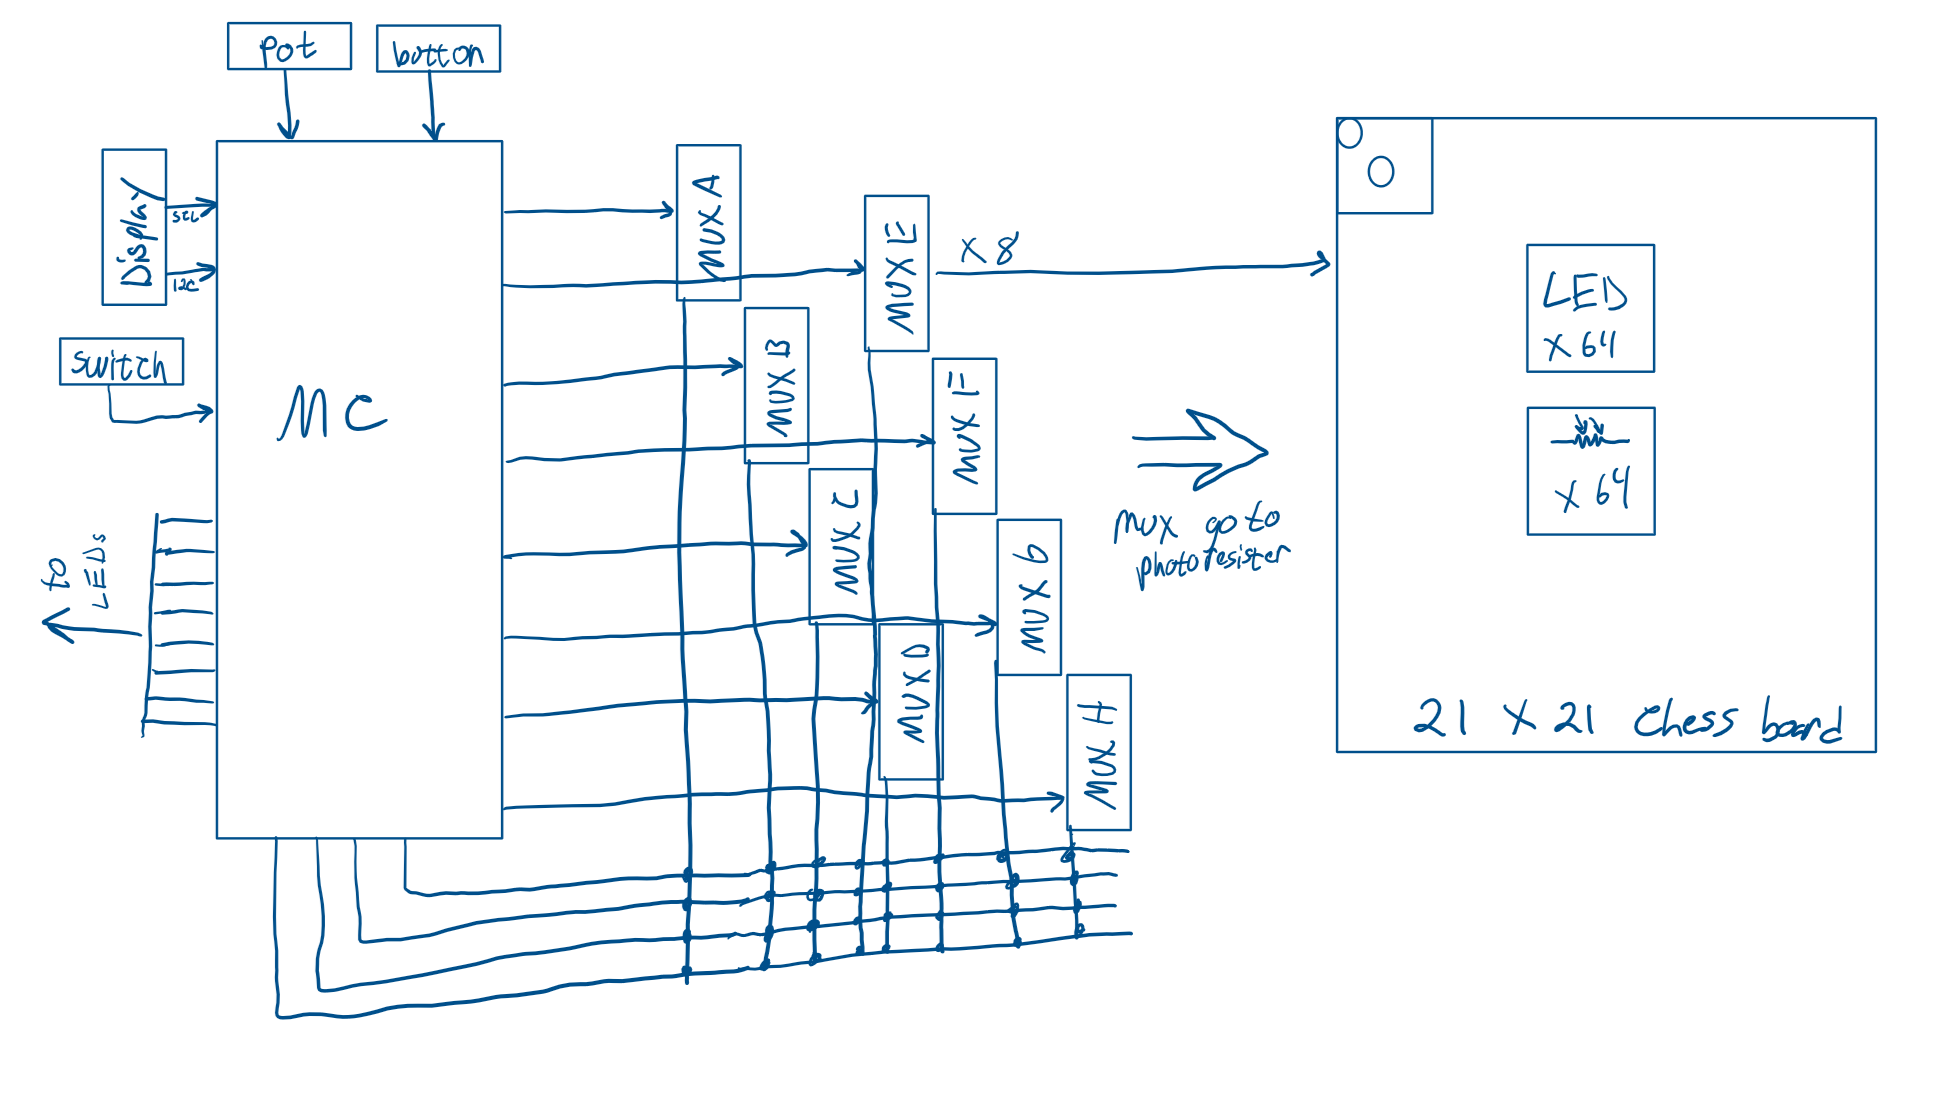
\includegraphics[width=\linewidth]{./Pics/System_Block_Diagram.PNG}
  \caption{System Block Diagram}
  \label{fig:SBD1}
\end{figure}

\subsection{Multiplexer Circuit Diagram} 
Figure \ref{fig:MSCD} shows the sudo circuit for Muxltiplexer A, the puzzle me chess project will consist of 8 Muxltiplexer one for each column A-H. Each of the Muxltiplexers will have 8 outgoing lines that will read Voltages levels from the rows \# 1-8. Each row will have one resister which will is set to be $~2M \Omega$ and one Photoresister in series. Each Photoresister has two modes a light and a dark mode. Equation (1) shows Mux input voltage at 3.29VDC and equation (2) shows Mux input voltage at 2.2VDC. 
\\


Assume Light; R = $500 \Omega$
\\


Assume Dark; R = $1M \Omega$


\begin{equation}
Light
$$ V = IR, 3.3VDC = I*(2M + 500)$\Omega$ $$
$$ I = 1.65$\mu$A, Vlight = 825$\mu$VDC, Mux input would see 3.299VDC if no piece on top of photoresister$$
\label{Light}
\end{equation}

\begin{equation}
Dark
$$ V = IR, 3.3VDC = I*3.3M$\Omega$ $$
$$ I = 1.1$\mu$A, Vdark = 1.1VDC, Mux input would see 2.2VD  if piece was placed on block$$
\label{Dark}
\end{equation}
\begin{figure}
  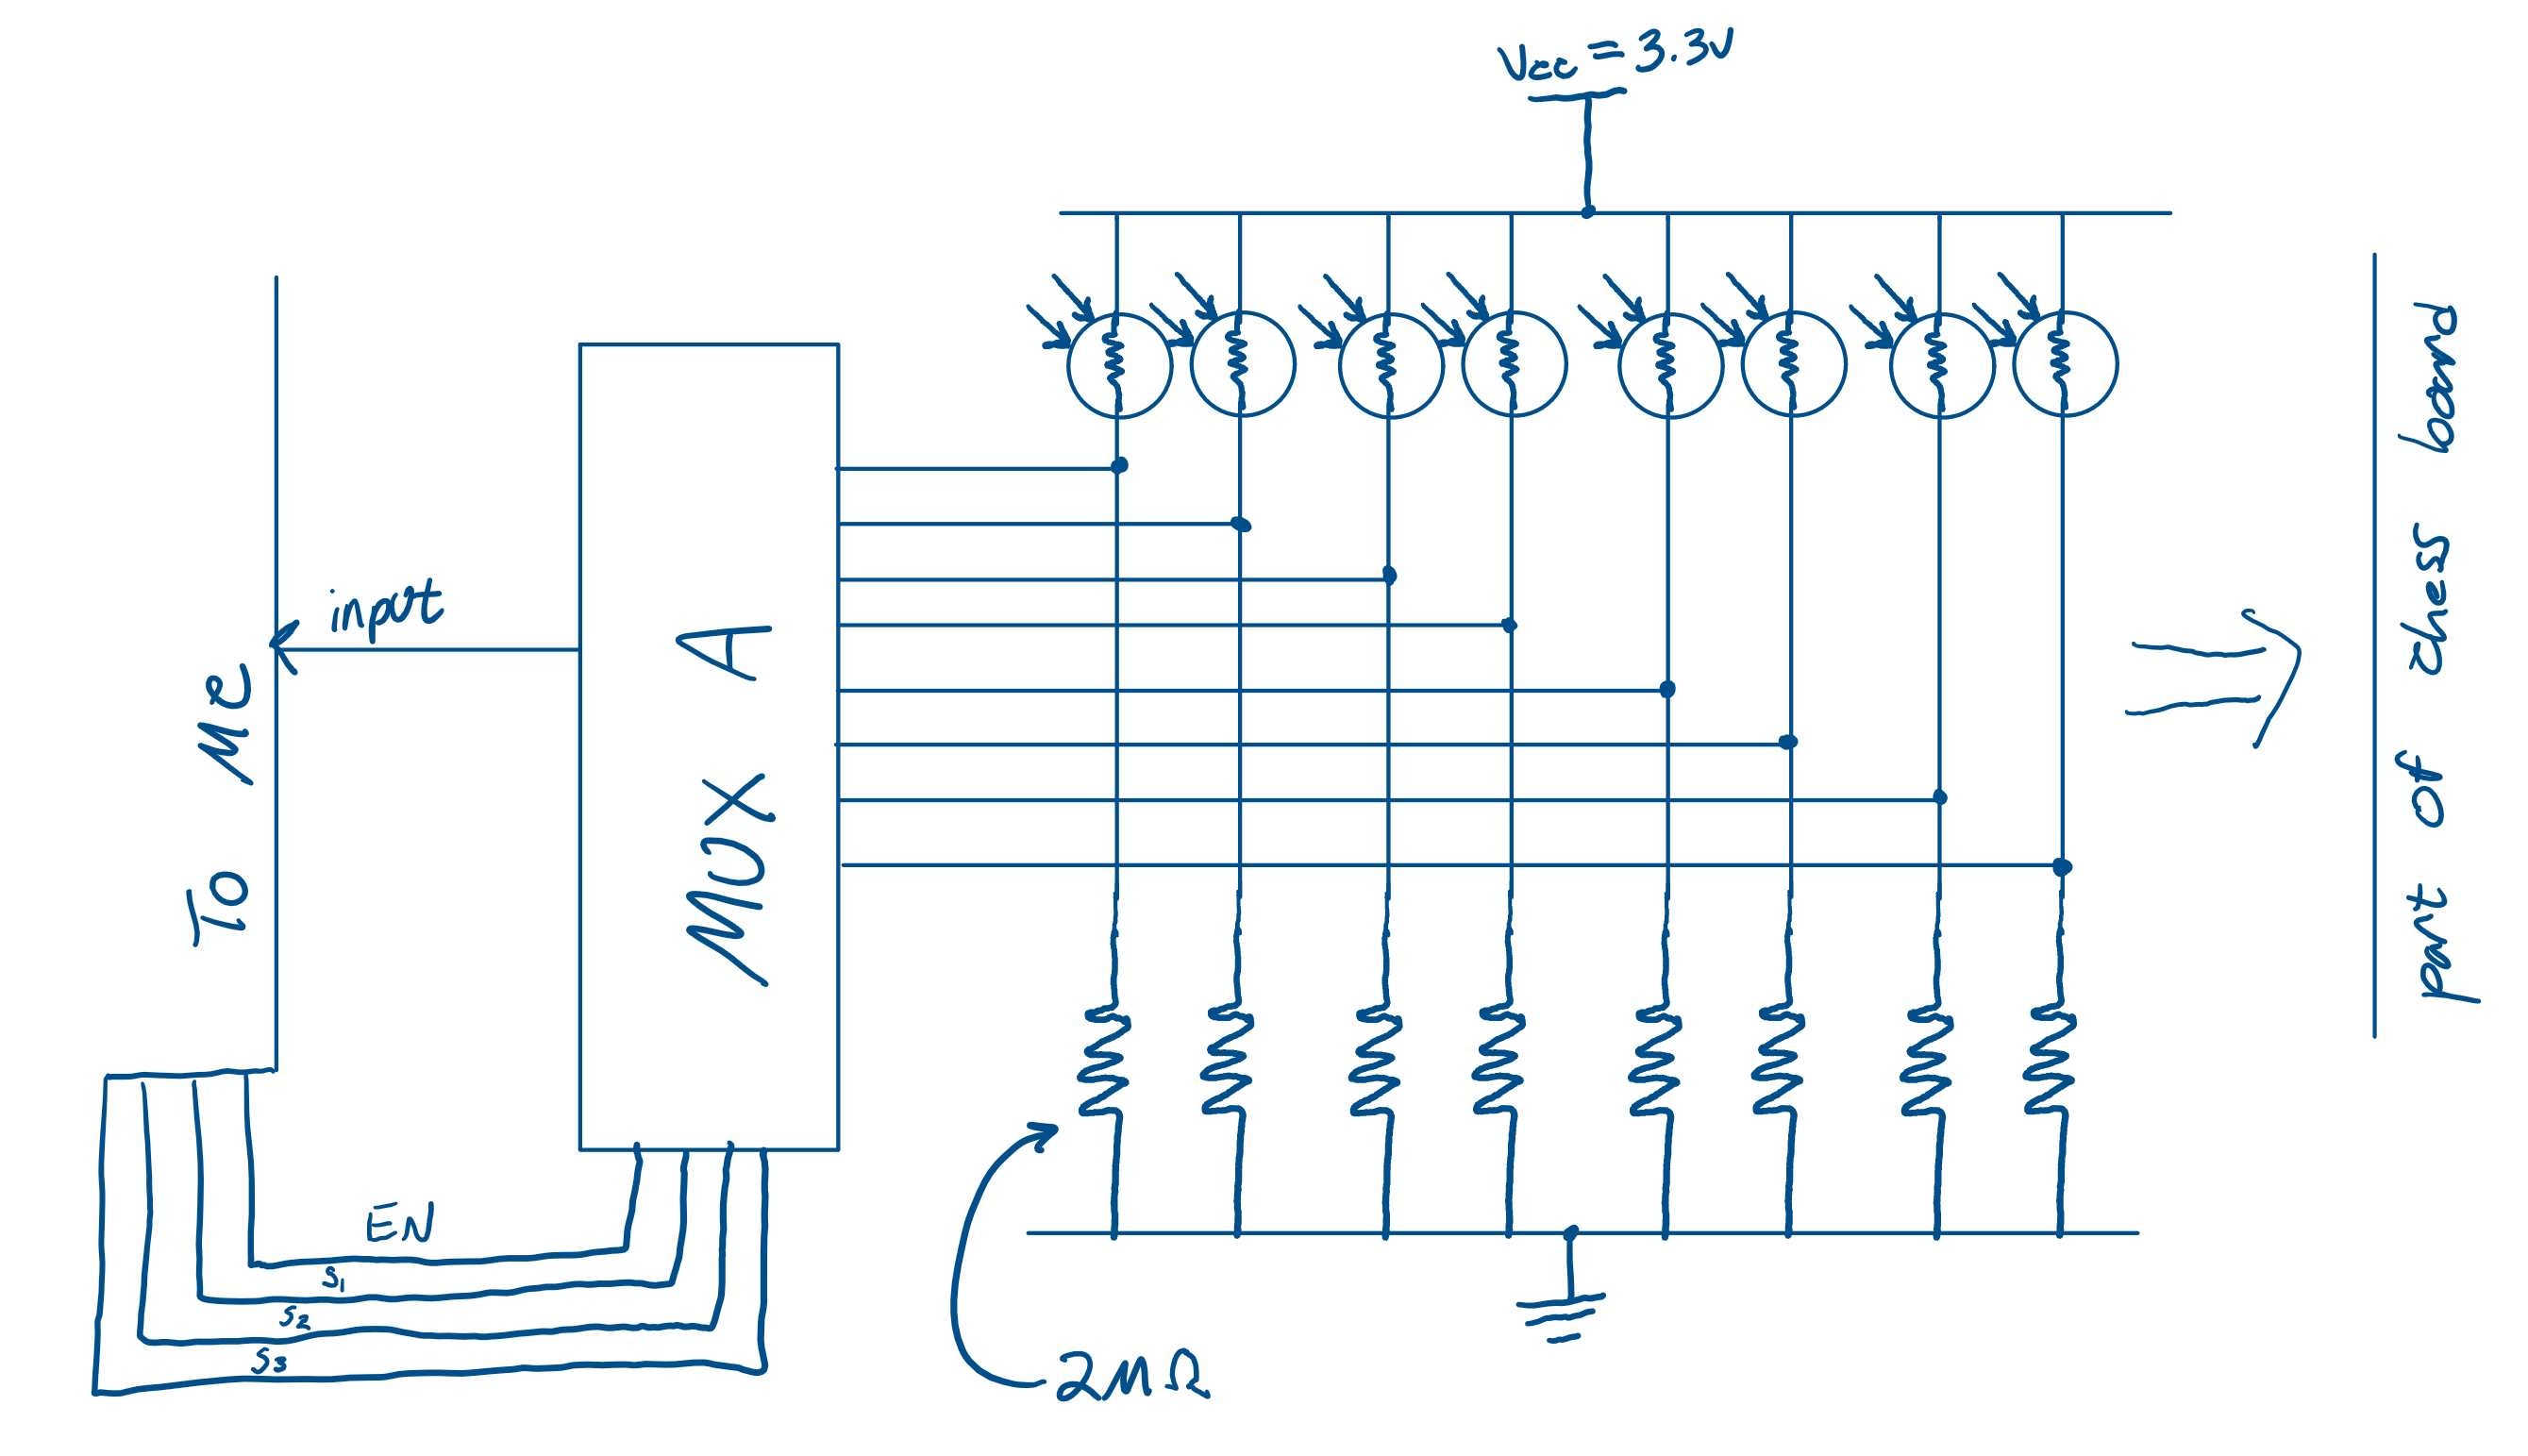
\includegraphics[width=\linewidth]{./Pics/Mux_sudo_circuit.PNG}
  \caption{Multiplexer Sudo Circuit Diagram}
  \label{fig:MSCD}
\end{figure}


\subsection{Code Flow Diagram}
Figure \ref{fig:CFD1} shows the code flow diagram. The code starts with the display showing the user to pick a puzzle which the user will use the potentiometer to select puzzle 1-3. After the Puzzle has been selected the display will show which puzzle the user selected and open that .csv file. The code will then mapp each space to a 2x2 matrix with a cell name attached. The code will then display to the user which to place each piece on which block. LEDs will also light up to quickly help the user where to place each piece. After each piece has been placed the code will shut off each LED light and display to the user which color to go first.  
\\


\noindent The code will have the ability to have the user use a button to light up LEDs to show the user the hint, and a switch to show the user the answer if they get stuck. If the wrong move is made on the chess board the code will have the ability to check each move and display if the move is correct or not. If the move is correct the display will show where the user needs to move the opponent piece so the user can continue the puzzle until completion. If the move is incorrect the user will be asked to place the piece back and try again. 

\begin{center}
\begin{figure}
  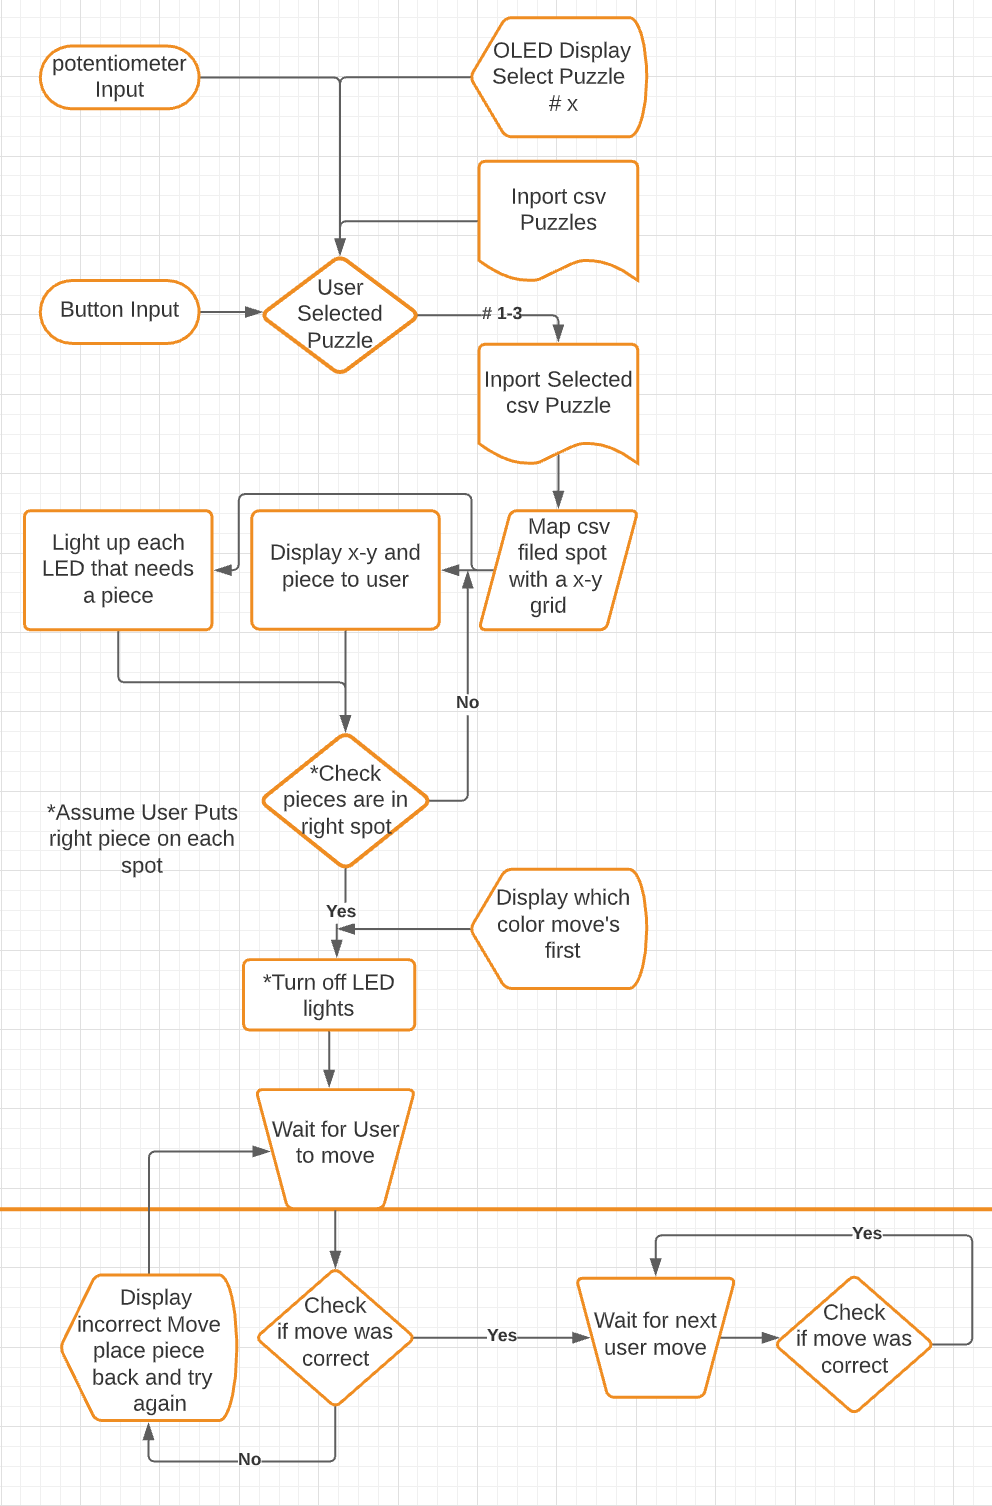
\includegraphics[width=17cm,height=21cm]{./Pics/Code_Flow_Diagram.PNG}
  \caption{Code Flow Diagram}
  \label{fig:CFD1}
\end{figure}
\end{center}

\section{Interface description}
The internal interface description consist of a display, switch, button, mulitiplexer, Potentiometer, and a SD Card. More information can be found in table \ref{tab:interface}. Charlieplexing is the method that will be used to turn on and off each LED that is needed to show the user where to put each piece, show hint and or show the answer. This equation to determine how many digital I/O pins needed to do this can be found in equation \eqref{Charlieplexiing}.

\begin{table}
\begin{center}
    \begin{tabular}{| l | l |}
    \hline
    Interface Description  & Description below\\ \hline
    Display & one SCL \@ 600MHz, one I2C  \\ \hline
    Mulitiplexer & 3 select digital I/0 pin, 1 enable digital I/O Pin, 8 Input digital I/O Pins \\ \hline 
    Switch & one digital I/O input pin \\ \hline
    Button & one digital I/O input pin \\ \hline
    Potentiometer & one analog PWM I/O input pin \\ \hline
    SD Card & I2C interface 4bit \\ \hline
    LEDs & 9 Digital I/O pins  to light up 64 LEDS \\ \hline
    \end{tabular}
    \caption{Shows the interface for Puzzle me Chess}
	\label{tab:interface}
\end{center}
\end{table}

\begin{equation}
Charlieplexing  
$$ Pins = $\frac{1}{2•}*(1+\sqrt{1+4*L}$; L=LED=64, Pins = 8.5$$
\label{Charlieplexiing}
\end{equation}

\section{Explanation of code}
The following sub sections will describe different parts of the current code as it stands on 02/18/2021. There will be a brief explanation of the code layout which uses reference \cite{stone}. Other code explanations will be outlined in Main, Display, SDcard,Button,and Potentiometer, see sections below for more information. 

\subsection{Code layout}
Figure \ref{fig:MCL1} shows the modulatory of the Puzzle me Chess code. Each component of the circuit has its function and for that it will get its own .h and .cpp files. As you can see in figure \ref{fig:MCL1}. This code modulatory is talked about in reference \cite{stone} and it states laying out the .h files to have a method that is used for one function. An example of this would be the Display having a method for initialization of the display, a print or draw function, and a clear function. This modulatory was done for each component a in the code and is clearly show in figure \ref{fig:MCL1}. For developing each method a .cpp file is used and these files will be discussed below in Listing \ref{main}, \ref{Display}, \ref{sdcard1}, \ref{button}, and \ref{Photentiometer}. All code below is current as of 02/18/2021 and is not finalized. 

\begin{figure}
  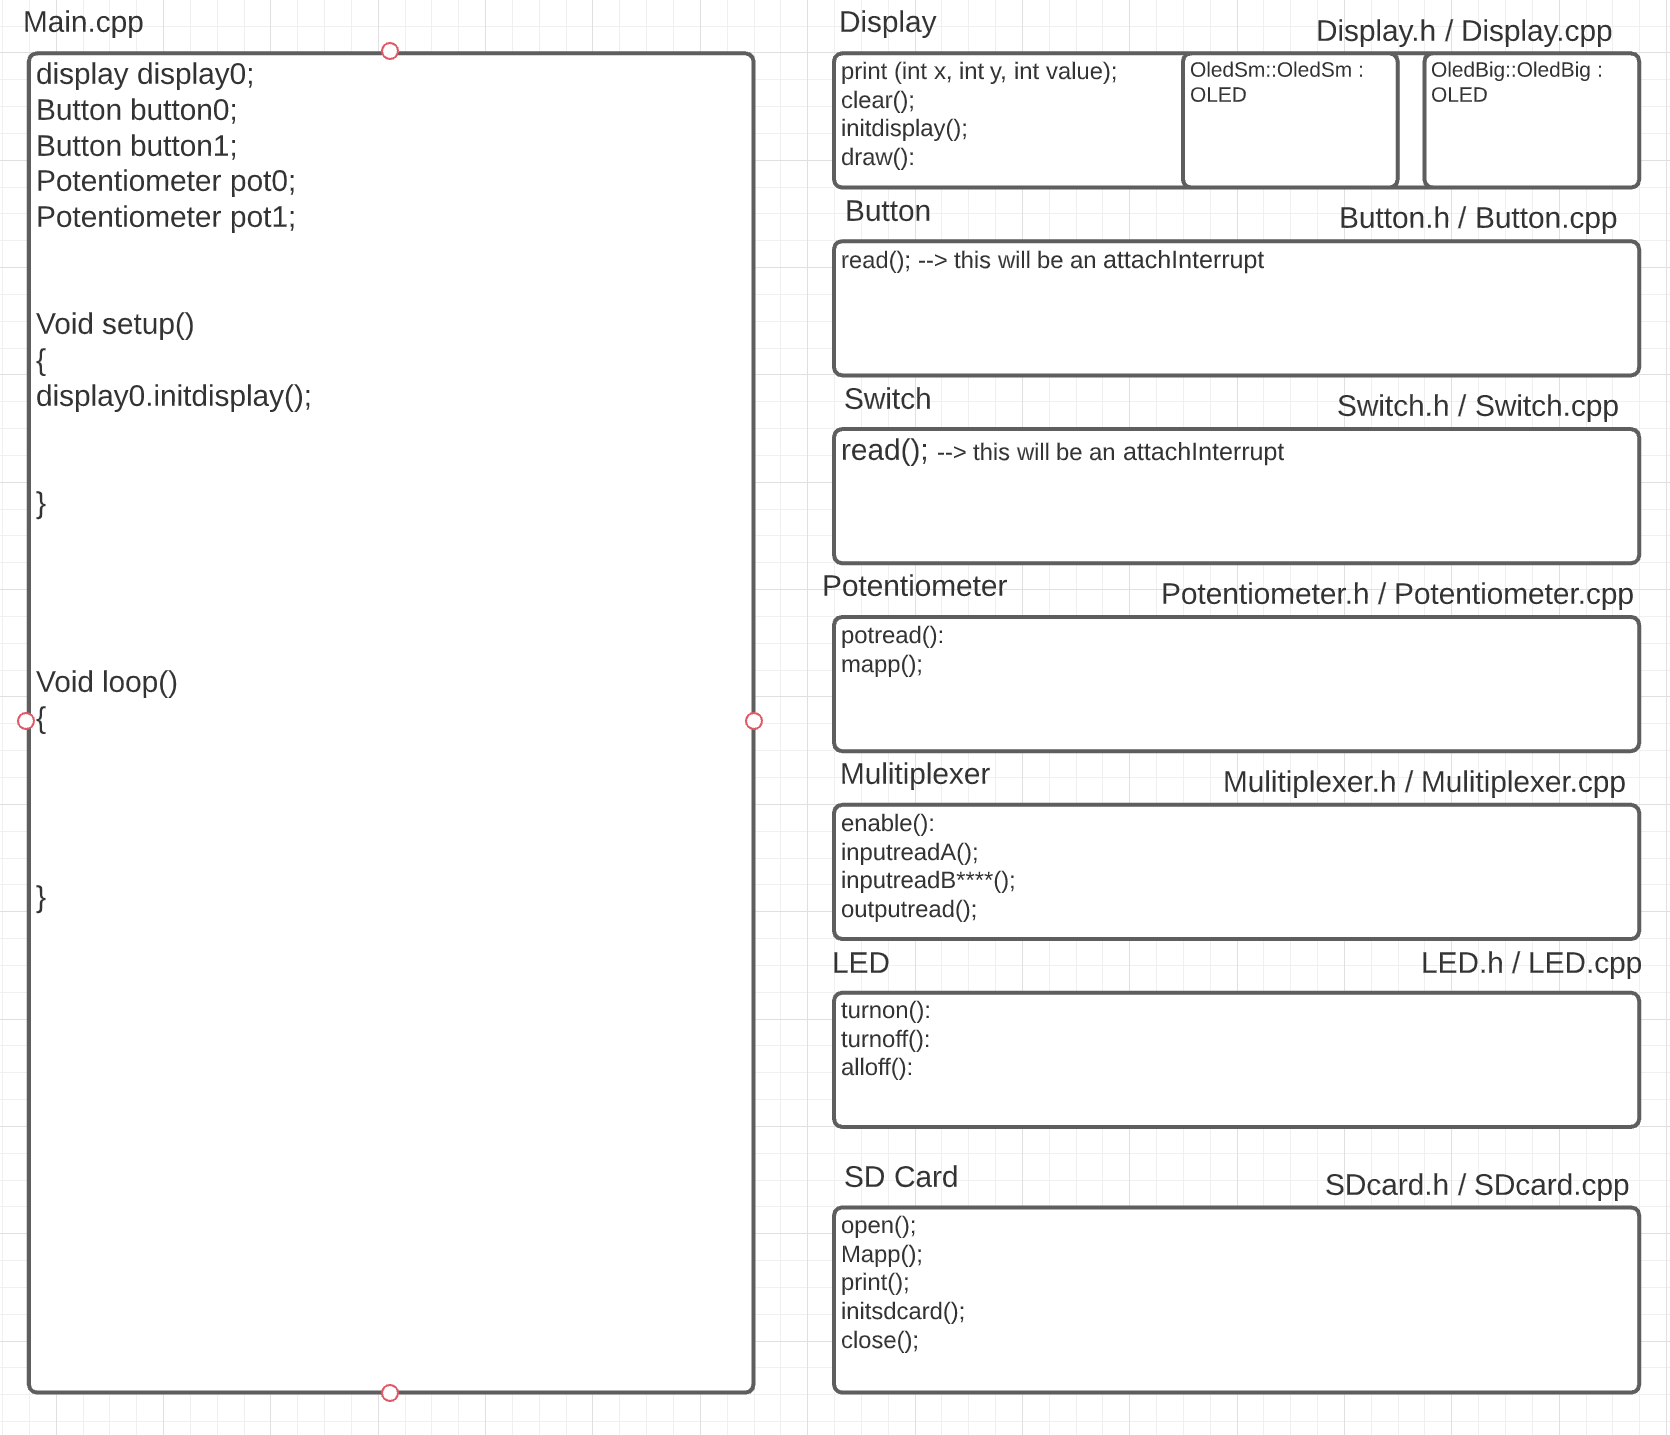
\includegraphics[width=\linewidth]{./Pics/code_layout.PNG}
  \caption{Module Code Layout}
  \label{fig:MCL1}
\end{figure}

\subsection{Main}
The main.cpp file in Arduino houses the main code.  Shown in Listing \ref{main} is the current main.cpp file code for Puzzle me Chess. At the top houses all the header files. Each header file is tied to its individual methods which are used in the individual .cpp files. Looking at Listing \ref{main} you have the header files and then come the declares. In the declare section there are method callers which grab the latest value of that method at any given time.   
\\

\noindent After the declares you call a function void setup() which generally would run one time and call most start up methods and initialization processes. Once the setup() function completes its run it then starts the main loop. In Arduino we use void loop() which loops every time it gets to the end but doesn't return any value. Currently I'm using two while loops which let the program pause as we wait for the user to enter in a value. The  first loop has the user select a puzzle and then the second loop tells the user which puzzle has been selected and then will open that .csv file. 

\begin{lstlisting}[caption={Puzzle me Chess - main.cpp file},label={main}]
//******************************************Declare****************************//
Display Display0; // Setting Object 0 for Display
SDcard SDcard0; 
Button Button0;
Potentiometer Potentiometer0; 
//******************************************Setup******************************//
void setup()
{
  Display0.int_display();
  SDcard0.int_SD();
//******************************************Inputs*****************************//
  Button0.init_button(); //setting D0 to button
  Potentiometer0.init_pot(); // setting A0 to pot
} // end setup

void loop()
{
//******************************************Declare****************************//
Button Button1;
Potentiometer Potentiometer2;
Display Display1;
//***************************************Start of Code*************************//
while (Button1.r_button() == 0)
{
  
  Potentiometer Potentiometer1; 
  Display1.print_select_puzzle(45, 30, Potentiometer1.r_pot());
}

delay(1000); //--> to allow for button press

while (Button1.r_button() == 0)
{
  Display1.print_user_puzzle(0,30, Potentiometer2.r_pot());
  SDcard0.open();
  break;
}
} //end void loop

\end{lstlisting}

\subsection{Display}
Listing \ref{Display} shows the .cpp file that holds all of the methods that are used within the main.cpp file and ran in void setup() and or void main(). Within the Display.cpp file there is the declare area which tells the code which display we are using and how to mapp the pins. After the declare the init.display() function is defined to start the display, followed by print.select.puzzle which shows the user which puzzle to select and the print.user.puzzle which will show the user which puzzle he/she selected. 

\begin{lstlisting}[caption={Puzzle me Chess - display.cpp file},label={Display}]
//******************************************Declare*****************************//
U8G2_SH1106_128X64_NONAME_F_HW_I2C u8g2(U8G2_R0, /* reset=*/U8X8_PIN_NONE);
//******************************************Setup******************************//
void Display::int_display()
{
    u8g2.begin(); // Start the Library code for the Display
} // end void int_display
//*****************************************Functions**************************//
void Display::print_select_puzzle(int x, int y, int value)
{   
    u8g2.clearBuffer();              // clear the internal memory
    u8g2.setFlipMode(0);             // Flips display 180 (1) = True
    u8g2.setFont(u8g2_font_9x18_tf); // choose a suitable font
    u8g2.drawStr(0, 12, "Select Puzzle");
    u8g2.drawStr(x, y, "#");
    u8g2.setCursor(60, 30); // set cursor location
    u8g2.print(value);
    u8g2.sendBuffer(); // transfer internal memory to the display
} // end void print_select_puzzle

void Display::print_user_puzzle(int a, int b, int value1)
{
u8g2.clearBuffer();
u8g2.setFlipMode(0);
u8g2.setFont(u8g2_font_9x18_tf); 
u8g2.drawStr(0, 12, "User Selected");
u8g2.drawStr(a, b, "#");
u8g2.setCursor(15, 30); 
u8g2.print(value1);
u8g2.drawStr(30, 30, "Puzzle");
u8g2.sendBuffer();
} // end void print_user_puzzle
\end{lstlisting}

\subsection{SDcard}
The SD card function is a big part of the Puzzle me Chess project. The goal of this code block is to mapp each of the 64 different spots on the .csv file to a spot on the chess board. After the mapping has been complete it will be used to light up each LED to show the user where to put each chess piece. The SD card code will need to be able to expect three different .csv files and mapp each to a different chess board layout and three completely different chess puzzles. 
\\

\noindent There are three main parts of the SD card code. The first part has you initialize the SDcard using code from reference \cite{sdcard}, second you need to open the file that was selected by the user, and lastly you need to mapp the open file to a chess board layout. Listing \ref{sdcard1} shows the second part of the SD card code. The code begins with opening a name of the .csv file and then it reads the file and prints the file on the serial terminal. After it prints the file it will close the file. Next I need to figure out how to mapp the SD card to a chess board layout. Look to use a Arduino - Multi-Dimensional Arrays to mapp the SD card to the chess board. 

\begin{lstlisting}[caption={Puzzle me Chess - SDcard.cpp file},label={sdcard1}]
void SDcard::open()
{
    if (!SD.begin(chipSelect))
    {
        while (true);
    }
    File dataFile = SD.open("1015704.CSV" ); //opening File T015704.csv

    // if the file is available, write to it:

    if (dataFile)
    {
        while (dataFile.available())
        {

            Serial.write(dataFile.read());
        }
        dataFile.close();
    }

    // if the file isn't open, pop up an error:

    else
    {
        Serial.println("error opening 1015704.CSV");
    }
}
\end{lstlisting}

\subsection{Button}
The button in Puzzle me Chess is used as a user interaction button. The user will have the ability to select which puzzle he or she would like to do and also when they are done setting up the chess board with the right pieces. Listing \ref{button} shows the .cpp file that is current used in the code. You have two methods. a initialize function that sets up the button to pin 0 as an input and a read button which sets the starting value of button to be equal to 1 and then to read the button and return a value of buttonstate1. 

\begin{lstlisting}[caption={Puzzle me Chess - button.cpp file},label={button}]
//*****************************************Functions**************************//
void Button::init_button()
{
pinMode(2, INPUT); // sets the digital pin 0 as input
} // end init_button

int Button::r_button()
{
int buttonstate1 = 1; 
buttonstate1 = digitalRead(button1);
return (buttonstate1);
} // end r_button
\end{lstlisting}

\subsection{Potentiometer}
The potentiometer is used as a user interaction point to have the user select which puzzle he or she would like to do. Listing \ref{Photentiometer}. shows the .cpp file for the potentiometer. The file has a simple read pot value that is also mapped to 1-3. So when the user turns the potentiometer the user will have three values to choose from. The file also has an initialize method which sets the potentiometer to AO on the microcontroller. 

\begin{lstlisting}[caption={Puzzle me Chess - Photentiometer.cpp file},label={Photentiometer}]
//*****************************************Functions**************************//
void Potentiometer::init_pot()
{
  pinMode(0, INPUT); // pin A0 mapped to an INPUT --> r_pot 
} // end init_pot

int Potentiometer::r_pot()
{
  int potmap1 = map(pot1, 0, 1023, 1, 3); // map values 1-3 
  return (potmap1);
} // end r_pot
\end{lstlisting}

\section{Material and resource requirements}
In this section we will discuss the list of items used in Puzzle me chess, the test equipment that will be used to test the code and test the circuit, and where we are ordering all components from and when we are due in. 

\subsection{List of Items (BOM)}
Table \ref{tab:BOM} shows the build of materials (BOM) used in the Puzzle me Chess project. 

\begin{table} 
\begin{center}
    \begin{tabular}{| l | l | c |}
    \hline
    Build of Material  & Item & Quantity \\ \hline
    Display & Teyleten Robot SongHe OLED Display Module 128x64 & 1 \\ \hline
    Mulitiplexer & Texas Instruments: part CD4051BE & 8 \\ \hline 
    Switch & Ximimark 2 Position SK12D07 3 Pin & 1 \\ \hline
    Button & Button Caps (square) & 1 \\ \hline
    Potentiometer & DGZZI 10k Trim Potentiometer with Knob: part 3386MP-103  & 1 \\ \hline
    SD Card & Micro Center 16GB Micro SD Card Class 10 Micro SDHC   & 1 \\ \hline
    LEDs & Novelty Place 100 Pcs 5mm White LED Diode Lights & 64\\ \hline
    Photoresister & eBoot  Photo Light Sensitive Resistor Light & 64\\ \hline
    2M resister & EDGELEC 100pcs 2M ohm Resistor 1/2w (0.5Watt) ±1\% & 64\\ \hline
    75 resister & EDGELEC 100pcs 75 ohm Resistor 1/2w (0.5Watt) ±1\%  & 64\\ \hline
    \end{tabular}
    \caption{Shows the BOM for Puzzle me Chess}
	\label{tab:BOM}
\end{center}
\end{table}

\subsection{Test equipment}
The Puzzle me Chess project consist of little test equipment needed to complete this project, however the ones that will be used are listing below. Testing circuits will be used to insure the to use a Charlieplexing circuit and the sudo mulitiplexer circuit layout before assembly of the entire circuit. 
\begin{itemize}
\item BK precision 2709B MM
\item Digital Analog Discovery 2
\subitem Oscilloscope
\subitem Logic Analyzer
\subitem Data Logger
\subitem Power Supply
\item 6236B Triple Output Power Supply 

\end{itemize}

\subsection{Ording from}
Table \ref{tab:ording} shows the current list of items that need to be ordered. The Display, Switch, Potentiometer and microcontroller have arrived already. 
\begin{table} 
\begin{center}
    \begin{tabular}{| l | l | c |}
    \hline
    Build of Material  & Website & Arrival \\ \hline
    Mulitiplexer & Digikey & March 12 \\ \hline 
    LEDs & Amazon & February 25 \\ \hline
    Photoresister & Amazon & February 25 \\ \hline
    2M resister & Amazon & February 25 \\ \hline
    75 resister & Amazon  & February 25 \\ \hline
    \end{tabular}
    \caption{Shows the BOM for Puzzle me Chess}
	\label{tab:ording}
\end{center}
\end{table}

\section{Development Plan and Schedule}
\subsection{Order of Development}
\begin{figure}
  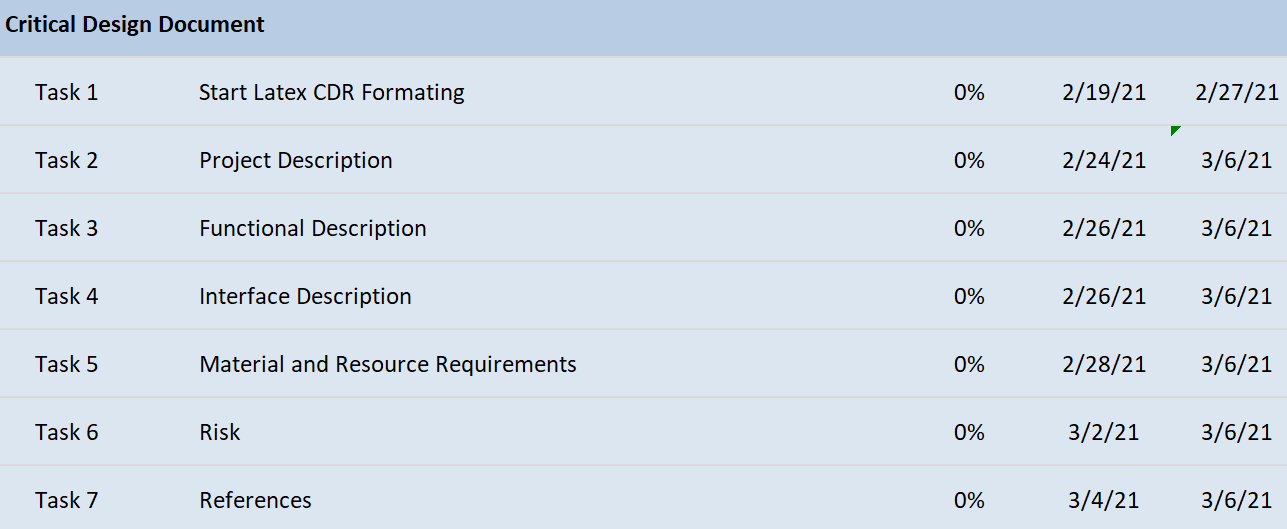
\includegraphics[width=\linewidth]{./Pics/Critical_design_document_gnatt.PNG}
  \caption{Critical Design Document}
  \label{fig:CDD}
\end{figure}


\begin{figure}
  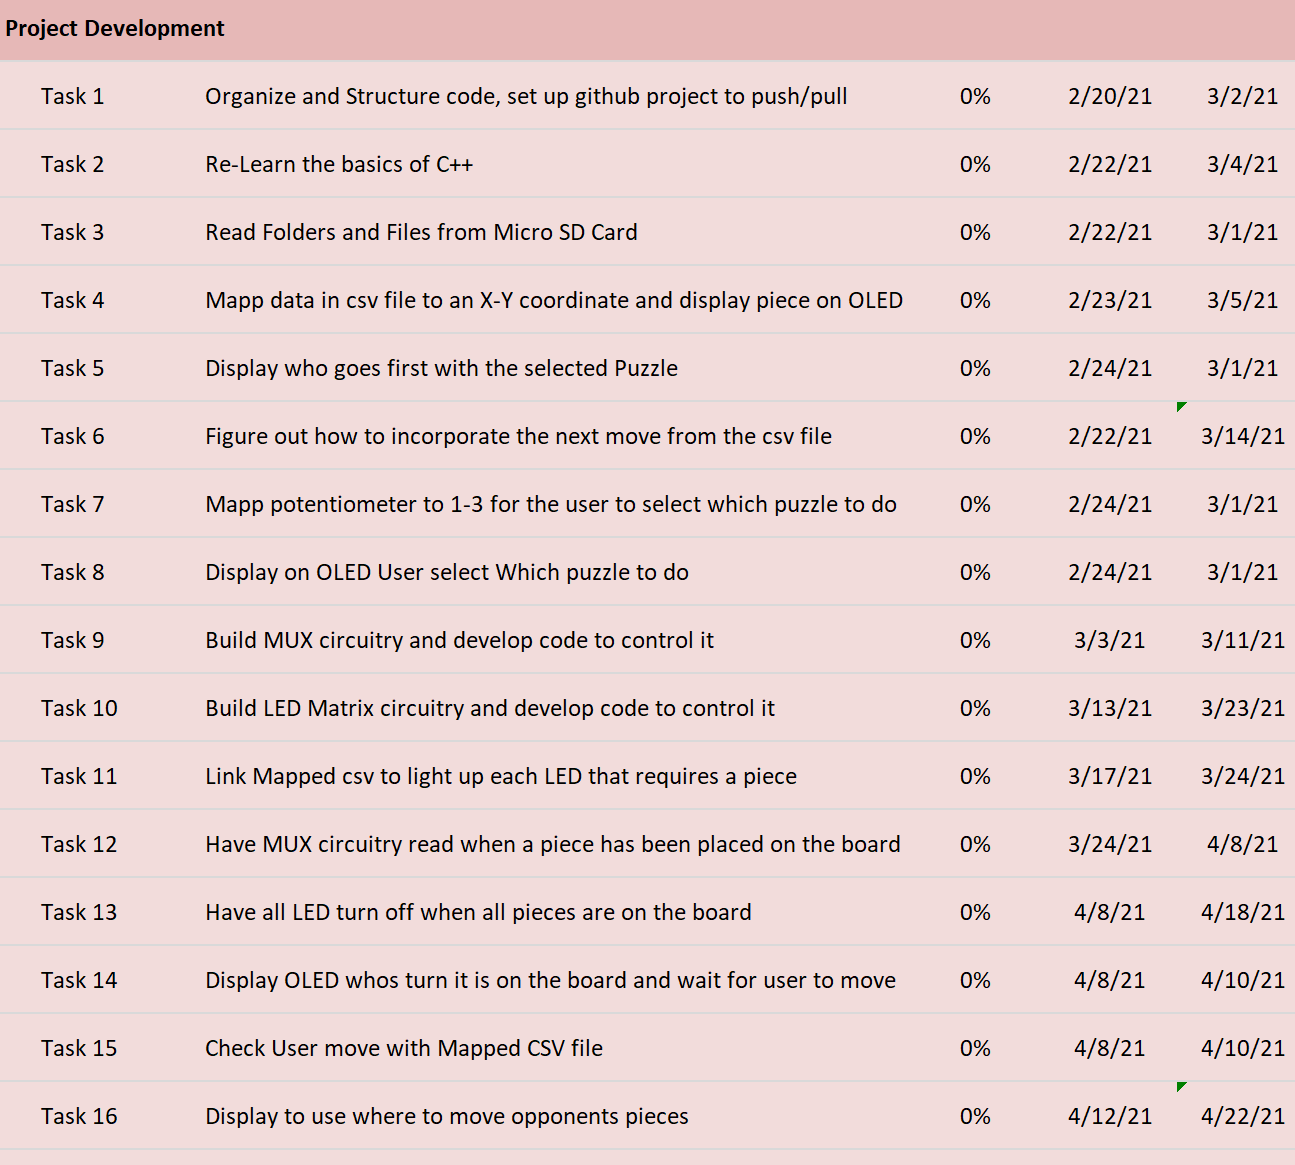
\includegraphics[width=\linewidth]{./Pics/Project_Development.PNG}
  \caption{Project Development}
  \label{fig:PD}
\end{figure}


\begin{figure}
  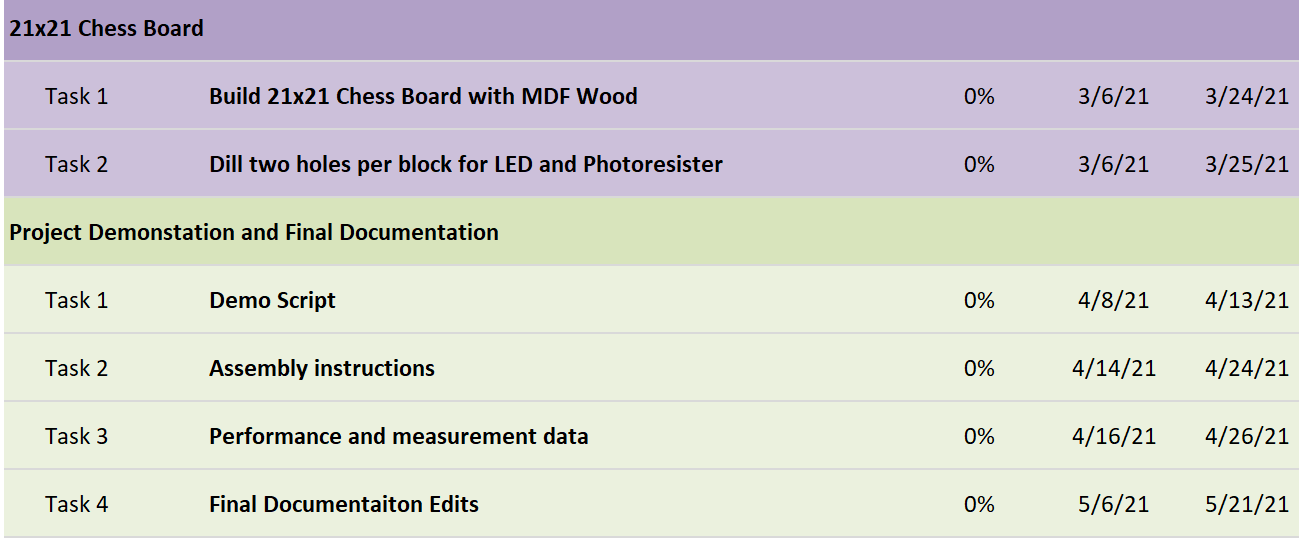
\includegraphics[width=\linewidth]{./Pics/Chess_Board_Project Demostation_Gnatt.PNG}
  \caption{Chest Board Development and Project Demonstration}
  \label{fig:CBPD}
\end{figure}



\subsection{Milestones and Schedule}
Below shows the completed and scheduled milestones for the Puzzle me Chess project. These milestones are taken from the course website.  
\begin{itemize}
\item Completed: 5 Jan	1st Meeting; Project Concept Development
\item Completed: 1  Feb	Project Concept Development 
\item Completed: 8 Feb	Submit Present Preliminary Design and Present to Class
\item 22 Feb	Submit Critical Design Document for Grade (no presentation)
\item 1 Mar - 3 May	Project Development \& Weekly Check-ins
\item 22 Mar	Holiday Break
\item 10 May	Project Demonstration
\end{itemize}

\subsection{Risk}


\begin{thebibliography}{2}
\bibitem{stone} 
Brain Stone. 
\textit{C++ Functions Modular Program Design}. (English) 
\textit{ Lecture presented at W 3.1, 3.2 }. 
Dublin City University Glasnevin, Dublin, 2001.

\bibitem{sdcard}
\textit{Team, T. (n.d.). Using the SD library to retrieve information over a serial port}.
\textit{ Retrieved February 18, 2021}, 
\textit{from https://www.arduino.cc/en/Tutorial/LibraryExamples/CardInfo}

\end{thebibliography}

\end{document}
